\begin{enumerate}[label=\thesection.\arabic*.,ref=\thesection.\theenumi]
\numberwithin{equation}{enumi}
\numberwithin{figure}{enumi}
%%
\item Let 
\begin{equation}
\mbf{y} = A\mbf{x} + \mbf{n},
\end{equation}
where 
\begin{align}
x &\in \brak{\mbf{s}_0,\mbf{s}_1}, 
\mbf{s}_0 = 
\begin{pmatrix}
1 
\\
0
\end{pmatrix},
\mbf{s}_1 = 
\begin{pmatrix}
0 
\\
1
\end{pmatrix}
\\
\mbf{n} &= 
\begin{pmatrix}
n_1
\\
n_2
\end{pmatrix},
n_1,n_2 \sim \gauss{0}{1}.
\end{align}
%
\item
\label{ch5_fsk}
Plot 
%
\begin{equation}
\mbf{y}|\mbf{s}_0 \text{ and } \mbf{y}|\mbf{s}_1
\end{equation}
%
on the same graph using a scatter plot.
%
\solution The following python code plots the scatter plot when $\mbf{x} = \mbf{s}_0$ and $\mbf{x} = \mbf{s}_1$ in Fig. \ref{fig:scatter_plt_y}
\begin{lstlisting}
codes/twoD/scatter_plot.py
\end{lstlisting}
\begin{figure}
\centering
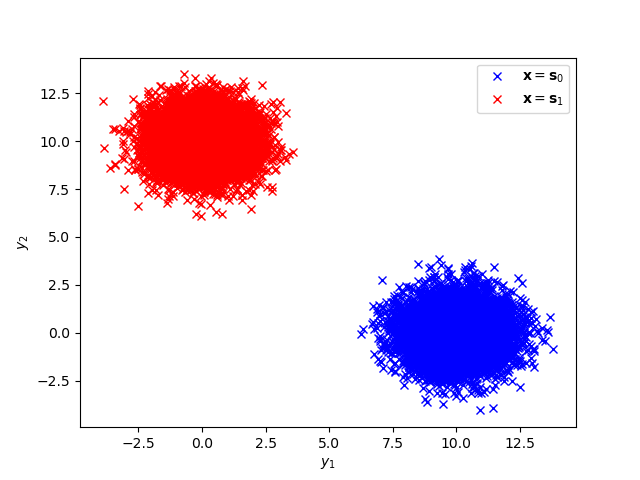
\includegraphics[width=\columnwidth]{./figs/twoD/scatter_plot.png}
\caption{Scatter plot of $\mbf{y} = \begin{pmatrix} y_1 \\ y_2 \end{pmatrix}$ for $A = 10$}
\label{fig:scatter_plt_y}
\end{figure}
%
%
\item
For the above problem, find a decision rule for detecting the symbols $\mbf{s}_0 $ and $\mbf{s}_1$.
\\
\solution The multivariate Gaussian distribution is defined as
%
\begin{multline}
\label{eq:multivariate}
p_{\mathbf{x}}(x_1,\dots,x_k)
\\
=\frac{1}{\sqrt{\brak{2\pi}^k\abs{\mbf{\Sigma}}}}\exp\cbrak{-\frac{1}{2}\brak{\mathbf{x}-\mbf{\mu}}^T\mbf{\Sigma}^{-1}\brak{\mathbf{x}-\mbf{\mu}}}
\end{multline}
%
where $\mbf{\mu}$ is the mean vector, $\mbf{\Sigma} = E\sbrak{\brak{\mathbf{x}-\mbf{\mu}}\brak{\mathbf{x}-\mbf{\mu}}^T}$ is the covariance matrix and $\abs{\mbf{\Sigma}}$ is the determinant of $\mbf{\Sigma}$.
For a bivariate gaussian distribution,
{\small
\begin{multline}
\label{eq:bivariate}
p(x,y)= \frac{1}{2\pi \sigma_x\sigma_y\sqrt{1-\rho^2}}\exp\lsbrak{-\frac{1}{2\brak{1-\rho^2}}}
\\
\times \rsbrak{\cbrak{\frac{\brak{x-\mu_x}^2}{\sigma_x^2}+\frac{\brak{y-\mu_y}^2}{\sigma_y^2}-\frac{2\rho\brak{x-\mu_x}\brak{y-\mu_y}}{\sigma_x\sigma_y}}}
\end{multline}
}
%
where
%
\begin{align}
%\mbf{\mu}=
&\mbf{\mu}=
\begin{pmatrix*}
\mu_x \\
\mu_y
\end{pmatrix*},
\mbf{\Sigma} = 
\begin{pmatrix*}%[r]
\sigma_x^2 & \rho\sigma_x\sigma_y \\
\rho\sigma_x\sigma_y & \sigma_y^2
\end{pmatrix*},\\
&\rho = \frac{E\sbrak{\brak{x - \mu_x}\brak{y-\mu_y}}}{\sigma_x\sigma_y}.
\end{align}
%
\begin{align}
    \mbf{y}|s_0 &= 
    \begin{pmatrix}
    A+n_1 \\
    n_2
    \end{pmatrix}\\
    \mbf{y}|s_1 &=  
    \begin{pmatrix}
    n_1 \\
    A+n_2
    \end{pmatrix}
    \end{align}
    Substituting these values in (\ref{eq:bivariate}),
    \begin{multline}
    \label{gauss_mutl_var1}
    p\brak{\mbf{y}|s_0} = \frac{1}{2\pi\sigma_{y_1}\sigma_{y_2}\sqrt{1-\rho_1^2}}\exp\lsbrak{-\frac{1}{2\brak{1-\rho_1^2}}}
    \\
    \times \rsbrak{\cbrak{\frac{\brak{y_1-A}^2}{\sigma_{y_1}^2}+\frac{\brak{y_2}^2}{\sigma_{y_2}^2}-\frac{2\rho_1\brak{y_1-A}\brak{y_2}}{\sigma_{y_1}\sigma_{y_2}}}}
    \end{multline}
    \begin{multline}
    \label{gauss_mutl_var2}
    p\brak{\mbf{y}|s_1} = \frac{1}{2\pi\sigma_{y_1}\sigma_{y_2}\sqrt{1-\rho_2^2}}\exp\lsbrak{-\frac{1}{2\brak{1-\rho_2^2}}}
    \\
    \times \rsbrak{\cbrak{\frac{\brak{y_1}^2}{\sigma_{y_1}^2}+\frac{\brak{y_2-A}^2}{\sigma_{y_2}^2}-\frac{2\rho_2\brak{y_1}\brak{y_2-A}}{\sigma_{y_1}\sigma_{y_2}}}}
    \end{multline}
    where,
    \begin{align}
    \label{rho_sig_val}
    \rho_1 = E[(y_1-A)(y_2)] &= E[n_1 n_2] = 0, \nonumber \\
    \rho_2 = E[(y_1)(y_2-A)] &= E[n_1 n_2] = 0, \nonumber \\
    \sigma_{y_1} = \sigma_{y_2} &= 1
    \end{align}
    For equiprobably symbols, the MAP criterion is defined as
    %
    \begin{align}
    \label{eq:map_bfsk_dec}
    p\brak{\vec{y}|s_0} &\dec{s_0}{s_1} p\brak{\vec{y}|s_1}
    \end{align}
    Using (\ref{gauss_mutl_var1}) and (\ref{gauss_mutl_var2}) and substituting the values from (\ref{rho_sig_val}),  we get
    \begin{align}
    (y_1 -A)^2 + y_2^2 \dec{s_1}{s_0} y_1^2 + (y_2 - A)^2
    \end{align}
    On simplifying, we get the decision rule is
    \begin{align}
    \label{eq:decision_rule}
    y_1 \dec{s_0}{s_1} y_2
    \end{align}
%    
\item
Plot 
\begin{equation} 
P_e = \pr{\hat{\mbf{x}} = \mbf{s}_1|\mbf{x} = \mbf{s}_0}
\end{equation}
with respect to the SNR from 0 to 10 dB.
\\
\solution
\begin{figure}
    \centering
    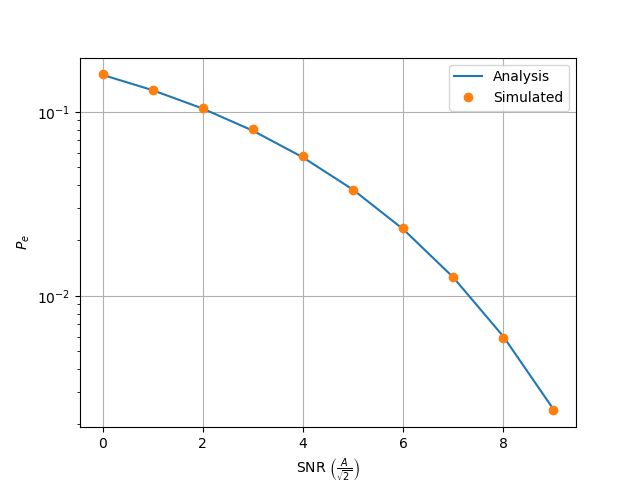
\includegraphics[width=\columnwidth]{./figs/twoD/ber_snr_plot.png}
    \caption{$P_e$ with respect to SNR from 0 to 10 dB}
    \label{fig:ber_snr_plot}
    \end{figure}
%
\item
Obtain an expression for $P_e$. Verify this by comparing the theory and simulation plots on the same graph.
\\
\solution 
\begin{align}
P_e = \pr{\hat{\mbf{x}} = \mbf{s}_1|\mbf{x} = \mbf{s}_0}
\end{align}
Given that $\mbf{s}_0$ was transmitted, the received signal is
\begin{align}
\mbf{y}|\mbf{s}_0 = \begin{pmatrix} A \\ 0 \end{pmatrix} + \begin{pmatrix} n_1 \\ n_2 \end{pmatrix}
\end{align}
From (\ref{eq:decision_rule}), the probability of error is given by 
\begin{align}
P_e &= \pr{y_1 < y_2 |\mbf{s}_0} = \pr{A+n_1 < n_2}\\
&= \pr{n_2 - n_1 > A}
\end{align}
Note that $n_2 - n_1 \sim \gauss{0}{2}$. Thus,
\begin{align}
P_e &= \pr{\sqrt{2}w > A}\\
\pr{w > \dfrac{A}{\sqrt{2}}}\\
\Rightarrow P_e &= \qfunc{\frac{A}{\sqrt{2}}}
\end{align}
where $w \sim \gauss{0}{1}$. The following code plots the $P_e$ curve in Fig. (\ref{fig:ber_snr_plot}).
\begin{lstlisting}
codes/twoD/ber_snr_plot.py
\end{lstlisting}
%
\end{enumerate}
